Entropy coding is a class of compression algorithms to occur last in the pipeline. These algorithms are given their name because their effectiveness is bounded by the entropy of incoming data. In the JPEG Compression Standard, a combination of Run-Length Encoding (RLE) and Differential Pulse Code Modulation (DPCM) is used, whose results are then fed into a Huffman Coder. The areas where these algorithms are used can be observed in Fig. \ref{fig:entropyjpeg}, with DPCM being used on the top left value of each chunk across all chunks in a channel (highlighted in green), and RLE being used on the remaining values in a single chunk, with the order in which values are encoded showed by the purple arrow.

Run-Length Encoding, as the name suggests, takes advantage of "runs" of data, storing the number of time a certain value or group of values repeats rather than storing every single repetition. In the case of the JPEG standard, RLE is used to group runs of zeroes in the AC components of DCT together, which appear in the data as a result of heavy quantization of DCT's high-frequency coefficients. So, each piece of data is encoded as a pair of integers, with the first being the number of preceding zeroes (up to 15) and the second being the following non-zero number (or a zero if there are 15 preceding zeroes). As an example, the string of values
\begin{equation*}
0,0,0,4,0,12,0,0,8,2.
\end{equation*}
would be encoded to
\begin{equation*}
(3,4);(1,12);(2,8);(0,2).
\end{equation*}
\begin{figure}
    \centering
    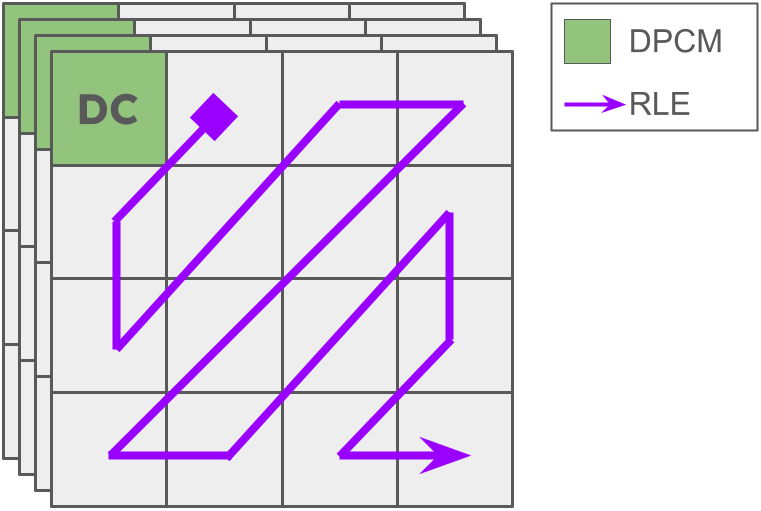
\includegraphics[width=0.8\linewidth]{methods/figures/dctentropyencode.png}
    \caption{Visual of different entropy encoding algorithms used for DCT as specified by JPEG Compression Standard.}
    \label{fig:entropyjpeg}
\end{figure}
While RLE is used for AC components, DPCM is used for DC components. At its core, DPCM is purely a differential coding algorithm, meaning it stores only the differences between values rather than the actual values themselves. This algorithm is most effective when adjacent values are correlated, which is the case for DC coefficients of adjacent image chunks (see "why images section"). By storing solely the differences between values, DPCM effectively stores values from the derivative function of the unencoded data, provided the unencoded data is correlated by some function itself. Thus, the efficiency of this algorithm depends much on the hope that the entropy of the derivative function is lower than that of the original function. Of course, to make data reconstruction possible, the first original value is stored, similarly to how integral calculation requires the constant $C$. To reconstruct the data, the differences are added to the first original value in sequence. For some sequence $[x]$ with difference sequence $[d]$:
\begin{equation}
\begin{split}
d_0 & = x_0 \\
d_1 & = x_1 - x_0 \\
d_{n} & = x_{n} - x_{n-1}
\end{split}
\end{equation}
and for reconstruction:
\begin{equation}
\begin{split}
x_0 & = d_0 \\
x_1 & = x_0 + d_1 \\
x_n & = x_{n-1} + d_n
\end{split}
\end{equation}

Related to DPCM is predictive coding, which uses previous values to predict future values and stores the difference between the actual value and the predicted value, known as prediction error. In cases when the data is highly correlated, predictions can be very accurate, causing the prediction error to be even smaller than differences calculated using DPCM, lowering entropy even further. Because of this, DPCM was substituted out for a linear predictive coder in this project pipeline. Similarly to DPCM, given some sequence $[x]$, we have predicted sequence $[p]$, with difference sequence $[d]$, where the difference sequence is stored in final data:
\begin{equation}
\begin{split}
p_n & = f(x_{n-1}, x_{n-2},...,x_{n-k}) \\
d_{n} & = x_{n} - p_n
\end{split}
\end{equation}
where function $f()$ is a linear regression model using $k$ previous values.